\documentclass{beamer}
\usetheme{Madrid}
\useoutertheme{infolines}
\beamertemplatenavigationsymbolsempty
\usepackage[utf8]{inputenc}
\usepackage{ragged2e} % \justifying
\usepackage{graphicx}
\usepackage{listings}
\graphicspath{{\files}}

% Default fixed font does not support bold face
\DeclareFixedFont{\ttb}{T1}{txtt}{bx}{n}{12} % for bold
\DeclareFixedFont{\ttm}{T1}{txtt}{m}{n}{12}  % for normal

% Custom colors
\usepackage{color}
\definecolor{deepblue}{rgb}{0,0,0.5}
\definecolor{deepred}{rgb}{0.6,0,0}
\definecolor{deepgreen}{rgb}{0,0.5,0}

\usepackage{upquote}
\usepackage{listings}

\lstset{mathescape,basicstyle=\ttfamily,breaklines=true,showstringspaces=false,literate={á}{{\'a}}1{é}{{\'e}}1{í}{{\'i}}1{ó}{{\'o}}1{ú}{{\'u}}1{ü}{{\"u}}1}

% Python style for highlighting
\newcommand\pythonstyle{\lstset{
language=Python,
basicstyle=\ttfamily,
otherkeywords={self},             % Add keywords here
keywordstyle=\ttb\color{deepblue},
emph={MyClass,__init__},          % Custom highlighting
emphstyle=\ttb\color{deepred},    % Custom highlighting style
stringstyle=\color{deepgreen},
showstringspaces=false            % 
}}

% Python environment
\lstnewenvironment{python}[1][]
{
\pythonstyle
\lstset{#1}
}
{}

% Python for external files
\newcommand\pythonexternal[2][]{{
\pythonstyle
\lstinputlisting[#1]{#2}}}

% Python for inline
\newcommand\pythoninline[1]{{\pythonstyle\lstinline!#1!}}

% Provide translations for blocks and primitives
\uselanguage{spanish}
\languagepath{spanish}
\deftranslation[to=spanish]{Example}{Ejemplo}
\deftranslation[to=spanish]{Definition}{Definición}

\title[(E)BNF y Expresiones Regulares]{Ayudantía Lenguajes de Programación}
\subtitle{(E)BNF y REGEX}
\author[RC/BG/AT]{\footnotesize Rodolfo Castillo Mateluna\and Benjamín Gautier Ortiz\and Andrés Tapia Olguín}
\institute[DI UTFSM]{U. Técnica Federico Santa María\\
Departamento de Informática}
\date{Segundo semestre 2017}

\setbeamertemplate{blocks}[default]
\setbeamertemplate{itemize items}[circle]
\setbeamertemplate{section in toc}{\inserttocsection}
\setbeamertemplate{subsection in toc}[square]

\begin{document}
\makeatletter
\setbeamertemplate{footline}
{
  \leavevmode%
  \hbox{%
  \begin{beamercolorbox}[wd=.333333\paperwidth,ht=2.25ex,dp=1ex,center]{author in head/foot}%
    \usebeamerfont{author in head/foot}\insertshortauthor\expandafter\beamer@ifempty\expandafter{\beamer@shortinstitute}{}{~~(\insertshortinstitute)}
  \end{beamercolorbox}%
  \begin{beamercolorbox}[wd=.333333\paperwidth,ht=2.25ex,dp=1ex,center]{title in head/foot}%
    \usebeamerfont{title in head/foot}\insertshorttitle
  \end{beamercolorbox}%
  \begin{beamercolorbox}[wd=.333333\paperwidth,ht=2.25ex,dp=1ex,right]{date in head/foot}%
    \usebeamerfont{date in head/foot}\insertshortdate{}\hspace*{2em}
    \insertframenumber{} / \inserttotalframenumber
    \hspace*{1em}
  \end{beamercolorbox}}%
  \vskip0pt%
}
\makeatother

	\begin{frame}[noframenumbering,plain]
		\titlepage
	\end{frame}
	
	\begin{frame}[noframenumbering,plain]{Contenidos}
		\tableofcontents
	\end{frame}
	
	\section{BNF}
	\subsection{Definición}
	
	\begin{frame}{Backus-Naur Form}
		\begin{definition}
       	\begin{itemize}
       	\item Es un lenguaje de marcado (no guarda estados) o metalenguaje.
        \item Se compone por elementos terminales y no terminales.
        \item Usualmente se utiliza una regla inicial principal, representado por un \texttt{S}$_0$
        \item Los elementos no terminales se expresan encerrados por \textless \textgreater.
        \item Se utilizan ``$|$" para indicar opciones.
       	\end{itemize}
		\end{definition}

    
	\end{frame}
	
	\subsection{Extended BNF}
	
\begin{frame}[fragile]{EBNF, a.k.a., Extended Backus-Naur Form}
		Agrega dos metacaracteres extra $=$ ``More Fun":
        \begin{itemize}
        \item $[$ \ $]$ Hace un s\'imbolo terminal o no terminal opcional, es decir, puede estar o no 							estar.
        \item  \{ \} Indica repetición de elementos, 0 o mas veces, la cantidad no se indica de manera 						expl\'icita.
        \item ejemplo: 
\begin{lstlisting}
<if_stmt> ::= if <condition> then <stmts> [else <stmts>] 
\end{lstlisting}
        \end{itemize} 
\end{frame}
		
	\subsection{Parse Tree}
	\begin{frame}{Lo que nos convoca: \emph{Parse Tree}}
		Nos permite detectar 2 cosas fundamentales del uso de (e)BNF, ambiguedad y determinar si una expresi\'on pertenece o no a la regla definida.
		Es necesario conocer la notación primeramente:\\

		\bigskip
        \begin{itemize}
        \item $\bigcirc$ : Terminales
        \item $\square$ : No Terminales
        \end{itemize}
	\end{frame}
    
\begin{frame}[fragile]{Ejemplo}
\begin{example}
Expresión:
\begin{lstlisting}
A := A * (B + C)
\end{lstlisting}
Gramática:
\begin{lstlisting}
<S$_0$>   : <id> := <exp> 
<id>  : A | B | C
<exp> : <id>+<exp> | <id>*<exp> | (<exp>)
      | <id>
\end{lstlisting}
\end{example}
\end{frame}

\begin{frame}{Ejemplo}
    \begin{figure}
    \centering
    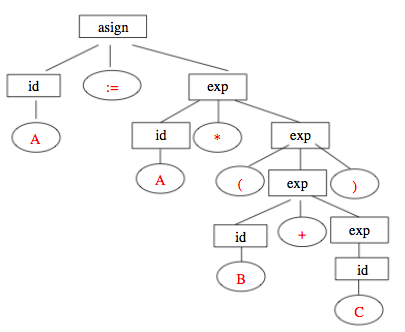
\includegraphics[width=0.8\textwidth]{parse}
    \end{figure}
\end{frame}

\subsection{Ambigüedad}
\begin{frame}[fragile]{Ambigüedad}
\begin{example}
\begin{lstlisting}
<S$_0$>   : <id> := <exp>
<id>  : A | B | C
<exp> : <exp>+<exp> | <exp>*<exp> | (<exp>)
      | <id>
\end{lstlisting}
\end{example}
\end{frame}

\begin{frame}{Ambigüedad}
\begin{figure}
\centering
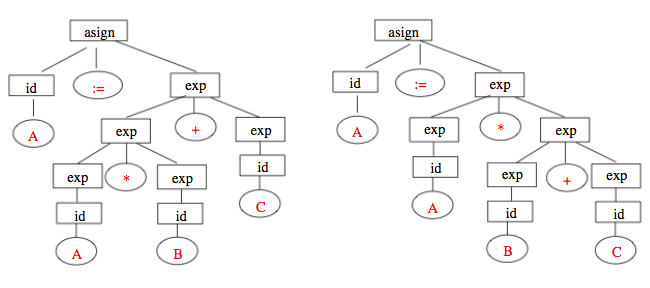
\includegraphics[width=\textwidth]{ambi}
\end{figure}
\end{frame}

\section{Expresiones regulares}
\subsection{Python: módulo \texttt{re}}

\begin{frame}[fragile]{Expresiones regulares en python, modulo \texttt{re}}
	\begin{itemize}
	\item El m\'odulo re posee funciones para trabajar con expresiones regulares y secuencias de caracteres en python.
    \item Con este modulo podemos crear objetos de tipo ``patrón" o objetos de tipo \emph{matcher}. Estos últimos son los que contienen la información de la coincidencia con el patrón en alguna secuencia.
    \item Algunos metacaracteres de importancia son:
    	\begin{itemize}
    	\item \$ calza el fin de string
        \item $[$ $]$ indica un conjunto, solo se elige un elemento.
        \item Rangos: \texttt{[a-z]}
        \item Rango negado: \texttt{[\textasciicircum a-z]}
        \item ``." coincide con cualquier caracter.
        \item \texttt{?} es opcional, es decir, cero o una vez.
        \item \texttt{+} es una o mas veces.
		\end{itemize}
    \end{itemize}
\end{frame}

\begin{frame}
		\begin{itemize}
        \item ...
          \begin{itemize}
          \item \texttt{*} es cero o mas veces.
          \item Ademas podemos crear grupos con paréntesis, o tambien podemos nombrar estos grupos:
              \begin{itemize}
              \item r'(a)([3-5]+)'
              \item (?P $<$letra$>$[a])(?P$<$numero$>$[3-5]+)
              \item Lo anterior nos servirá para obtener los grupos mediante la funcion \texttt{group()}
              \end{itemize}
          \end{itemize}
          \end{itemize}
\end{frame}

\begin{frame}[fragile]{...Uso de re en Python}
	\begin{itemize}
    \item Lo primero es definir una expresion regular o un patron:
\begin{lstlisting}
patron = re.compile('(a)([3-5]+)')
\end{lstlisting}
	\item Luego tenemos un objeto de tipo patron, usado para manejar expresiones regulares.
    \item Existe una serie de funciones como \texttt{match, search, findall}, que requieren de un patron compilado para ser usados sobre alguna entrada de texto. Por ejemplo:
\begin{lstlisting}
string = 'a345'
objeto = patron.match(string)
objeto.group(0) -> 'a345'
objeto.group(1) -> 'a'
objeto.group(2) -> '345'
\end{lstlisting}
	\item En \texttt{objeto} se encuentra el matching del patron con una entrada o string.
	\end{itemize}
	
\end{frame}
    
    
\end{document}












